\documentclass{article}
\usepackage[utf8]{inputenc}
\usepackage{graphicx}
\graphicspath{Figure_1.png}

\title{AlgLin - Principal Component Analysis}
\author{João Pedro Paiva Cardoso, Marcos Paulo Sousa Santos}
\date{December 2022}

\begin{document}

\maketitle

\section{O Dataset}
\par
Selecionamos um dataset do Instituto Nacional de Diabates e Doenças Digestórias e Renais (Reino Unido) que foi utilizado em um estudo que visava prever casos de diabetes utilizando dados do sangue dos pacientes.\par 
Este dataset consiste em diversas variáveis médicas como IMC, nível de insulina, idade etc e de uma váriavel alvo, Outcome (resultado). Outcome = 1 representa resultados positivos (o paciente possui diabetes) e Outcome = 0 representa resultados negativos (o paciente não possui diabetes).
\section{O Algoritmo}
Primeiro, para normalizar os dados, obtivemos a média (mean) e a subtraímos do total de dados. Dessa forma deixando os valores das colunas mais uniformes.
\begin{verbatim}
    mean = np.mean(data,axis=0)
    meanReducedData = data - mean
\end{verbatim}
Então, calculamos a matriz de covariância e a transpomos pois o algoritmo estava trabalhando com base nas linhas e não nas colunas:
\begin{verbatim}
    covMatrix = np.cov(MeanReducedData.T)
\end{verbatim}
Com isso já podemos calcular os autovetores (eigVec) e autovalores (eigVal):
\begin{verbatim}
    eigVal,eigVec = np.linalg.eig(covMatrix)
\end{verbatim}
Sabendo os autovalores, os ordenamos do maior para o menor
\begin{verbatim}
    eigVal = np.array(np.sort(eigVal))[::-1]
\end{verbatim}
Descobrimos assim que os maiores autovalores são 1.34565776e+04 e 9.32085966e+02, que correspondem as colunas Pregnancies (nº de gravidez) e Glucose (glicose) respectivamente.
Por fim, basta representar estas colunas em um gráfico.
\begin{verbatim}
    sns.lineplot(x="Pregnancies",y="Glucose",data=data,hue="Outcome")
    plt.show()
\end{verbatim}
\begin{figure}
    \centering 
    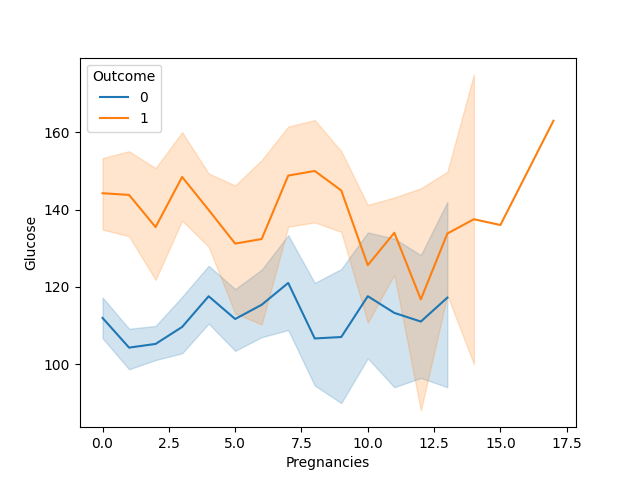
\includegraphics{Figure_1.png}
    \caption{Gráfico dos Maiores Autovalores}
    \label{fig:my_label}
\end{figure}
Observando o gráfico a seguir vemos que conforme a Glicose e as Gravidezes aumentam, o Outcome 1 (resultado positivo) é maior. Ou seja, são as melhores variáveis para se analisar.
\end{document}
